% !TEX program = xelatex
\documentclass[10pt,aspectratio=43,mathserif]{beamer}		
%设置为 Beamer 文档类型,设置字体为 10pt,长宽比为16:9,数学字体为 serif 风格

%%%%-----导入宏包-----%%%%
\usepackage{seu}
\usepackage{xeCJK}
\usepackage{amsmath,amsfonts,amssymb,bm}
\usepackage{color}
\usepackage{graphicx,hyperref,url}
\usepackage{subfigure}	
%%%%%%%%%%%%%%%%%%


%%%%-----设置字体-----%%%%
%Windows和Mac OS下都可用
\setsansfont{Helvetica}

%\setsansfont{Times New Roman}

%仅Windows可用
%\setCJKmainfont{Hiragino Sans GB W3}

%仅Mac OS下可用
%\setCJKmainfont{Songti SC}




%设置 Beamer 主题
\beamertemplateballitem


\AtBeginSection[]
{
  \begin{frame}<beamer>
    \frametitle{\textbf{目录}}
    \textbf{\tableofcontents[currentsection]}
  \end{frame}
}


%%%%----首页信息设置----%%%%
\title[RF-based Blood Donor Recruitment]{\fontsize{13pt}{18pt}\selectfont {基于随机森林的献血招募模型}}
%\subtitle{\fontsize{9pt}{14pt}\selectfont \textbf{基于随机森林的献血招募模型}}			
%%%%----标题设置


\author[Zixing Song]{
  宋子星 \\
  %{\small {songzixing@seu.edu}
  }

%%%%----个人信息设置

\institute[SEU]{
  东南大学计算机科学与工程学院\\
  }
%%%%----机构信息

\date[\today]{
 \today}
%%%%----日期信息


\begin{document}

\begin{frame}
\titlepage
\end{frame}				%生成标题页



\section*{目录}

		\begin{frame}
		\frametitle{\textbf{目录}}
		\textbf{\tableofcontents}
		\end{frame}				%生成提纲页

\section{背景}

		\begin{frame}
            \frametitle{\textbf{背景}}

            \begin{block}{\textbf{现状与意义}}
                \begin{itemize}
                    \item 医疗领域:当前献血招募主要采取人力招募方式
                    \item 计算机领域:机器学习技术迅猛发展
                    \item 献血招募 + 机器学习 $\Rightarrow$ 提升招募精度 + 降低招募成本 ?
                \end{itemize}
            \end{block}

            \begin{figure}[!t]
                \centering 
                \subfigure{
                    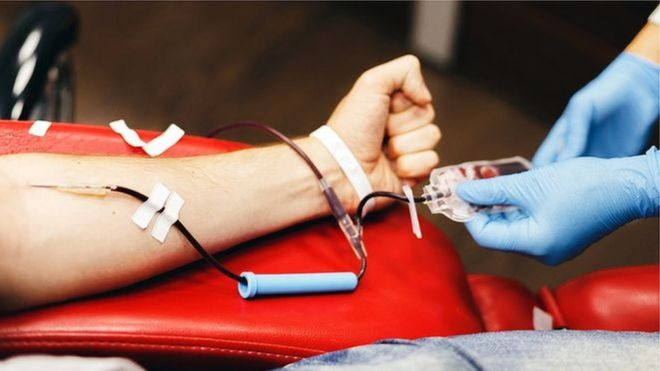
\includegraphics[width=2in]{figures/blood_donation.jpg}
                }
                \subfigure{
                    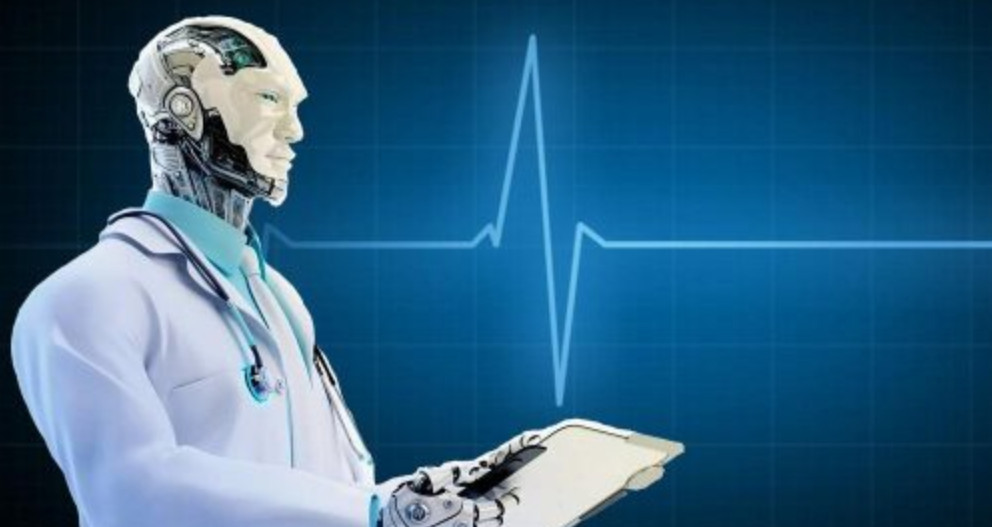
\includegraphics[width=2in]{figures/medical_AI.jpg}
                }
            \end{figure}

    \end{frame}

    \begin{frame}
        \frametitle{\textbf{研究问题}}
        \begin{figure}[!t]
            \centering 
            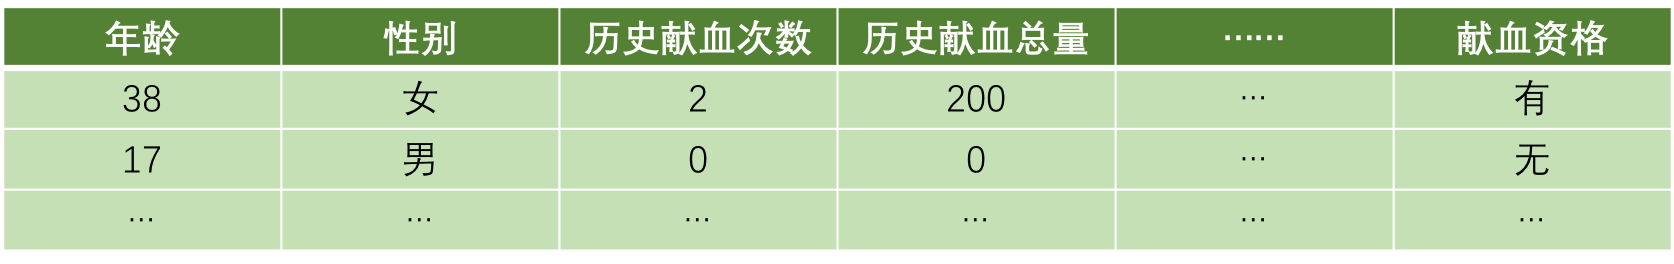
\includegraphics[width=4in]{figures/samples.png}
        \end{figure}
        
        \begin{figure}[!t]
            \centering 
            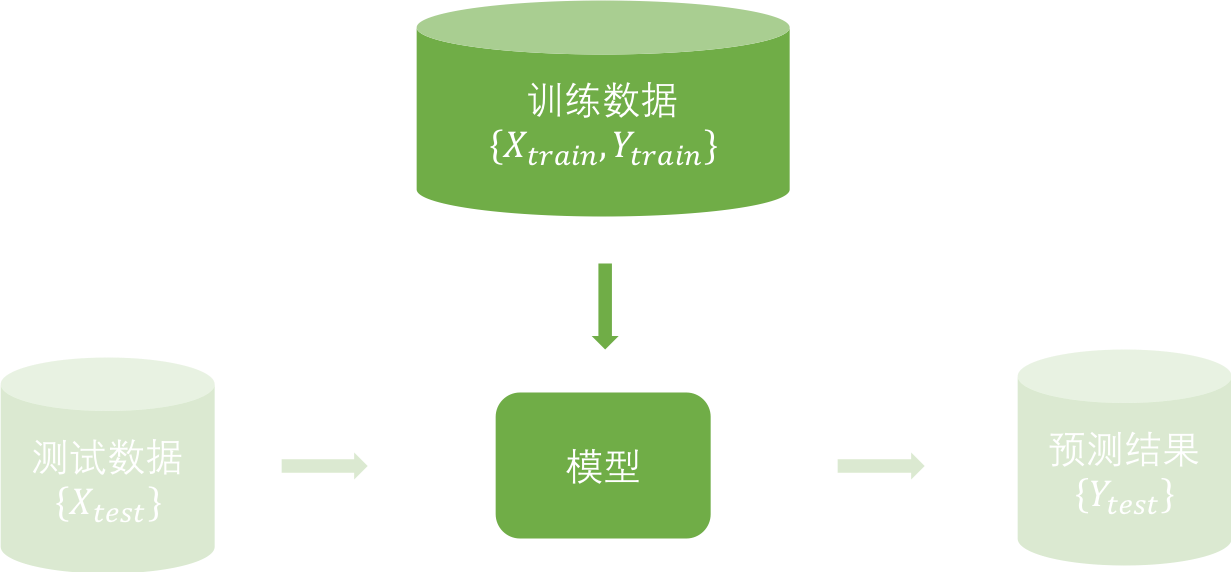
\includegraphics[width=4in]{figures/training1.png}
        \end{figure}

    \end{frame}

    \begin{frame}
        \frametitle{\textbf{研究问题}}
        \begin{figure}[!t]
            \centering 
            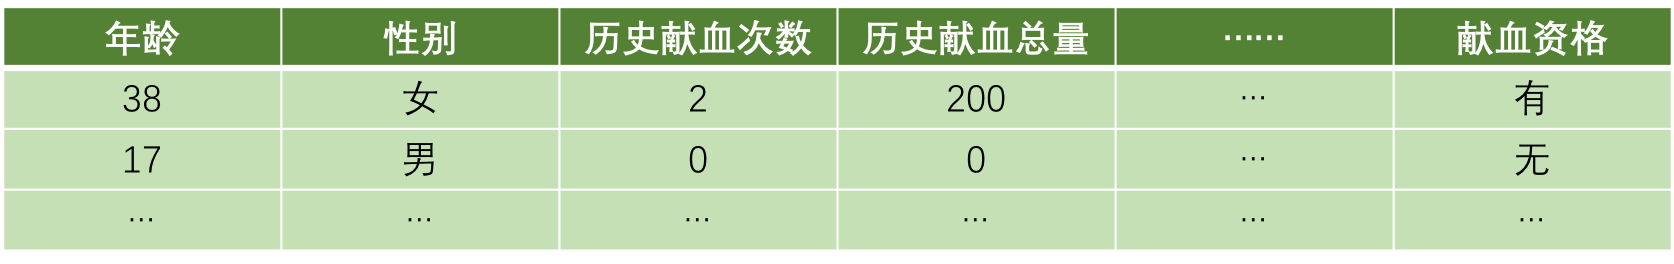
\includegraphics[width=4in]{figures/samples.png}
        \end{figure}
        
        \begin{figure}[!t]
            \centering 
            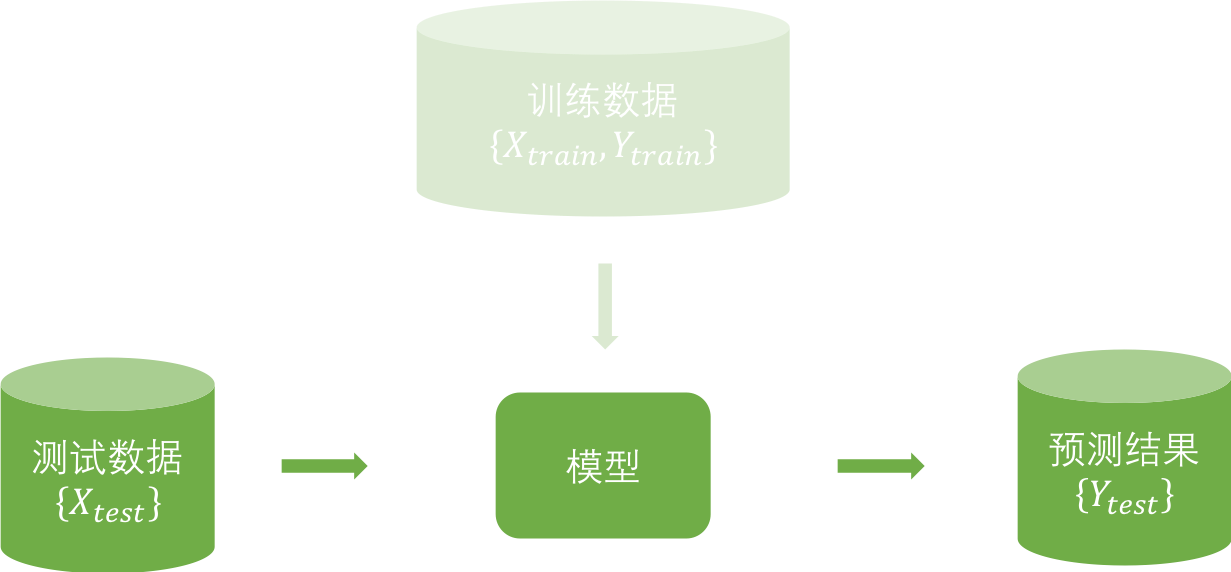
\includegraphics[width=4in]{figures/testing1.png}
        \end{figure}

    \end{frame}

\section[理论]{随机森林理论}

		\begin{frame}
		  \frametitle{\textbf{集成学习(Ensemble Learning)}}
            \begin{figure}[!t]
            \centering
            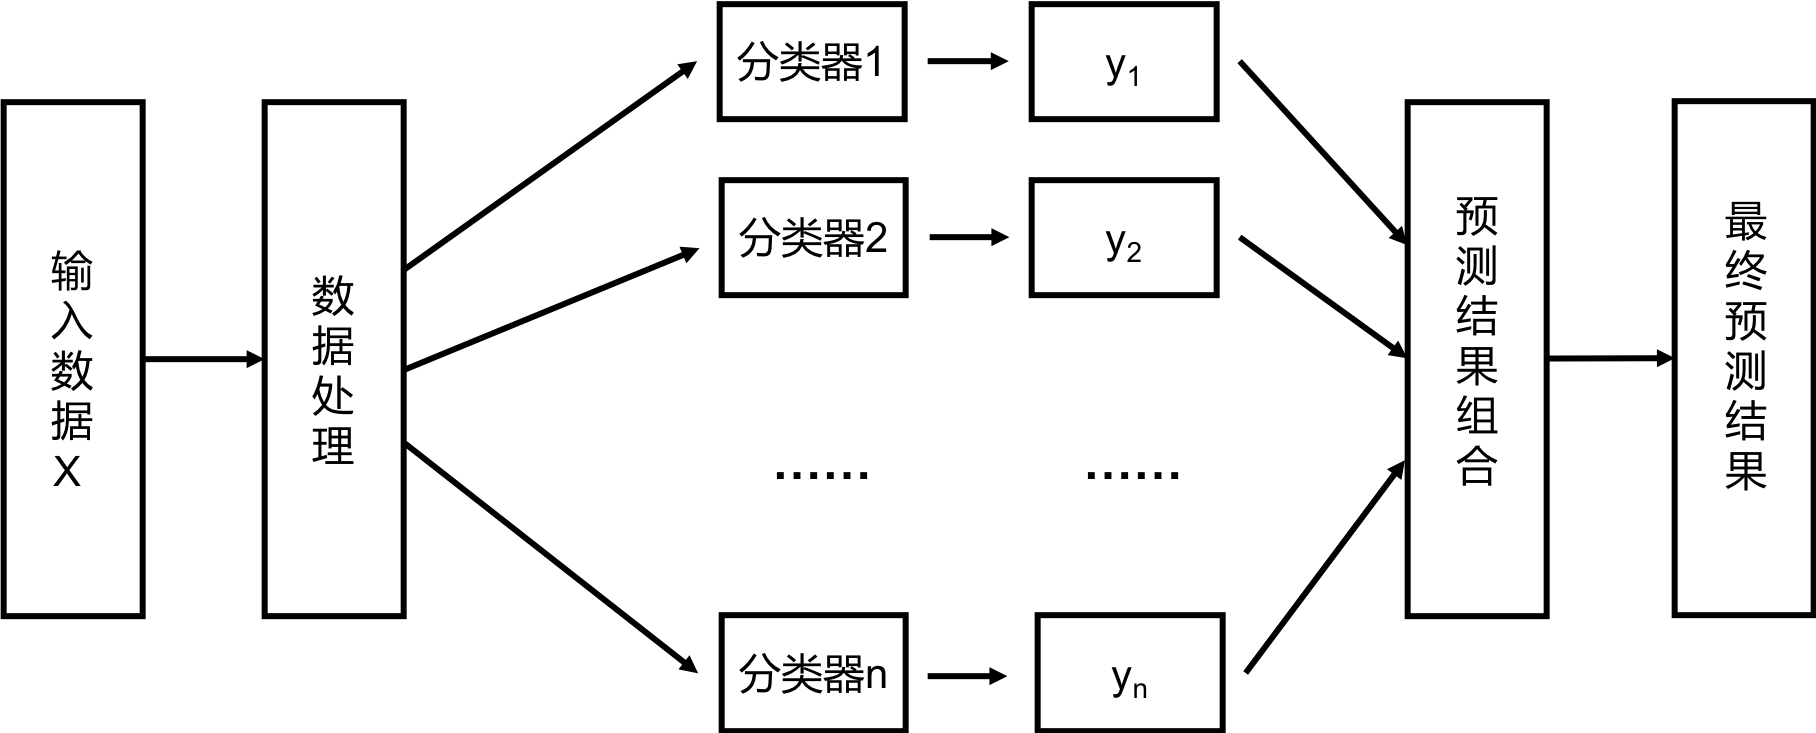
\includegraphics[width=4in]{figures/el.png}
            \caption{集成学习流程框架}
            \label{el}
            \end{figure}
            \textbf{集成学习}是指用于训练多个学习器并组合其输出,可以将其视为“决策委员会”的投票决策结果。
		\end{frame}

		\begin{frame}
		  \frametitle{\textbf{Bagging}}
            \begin{figure}[!t]
            \centering
            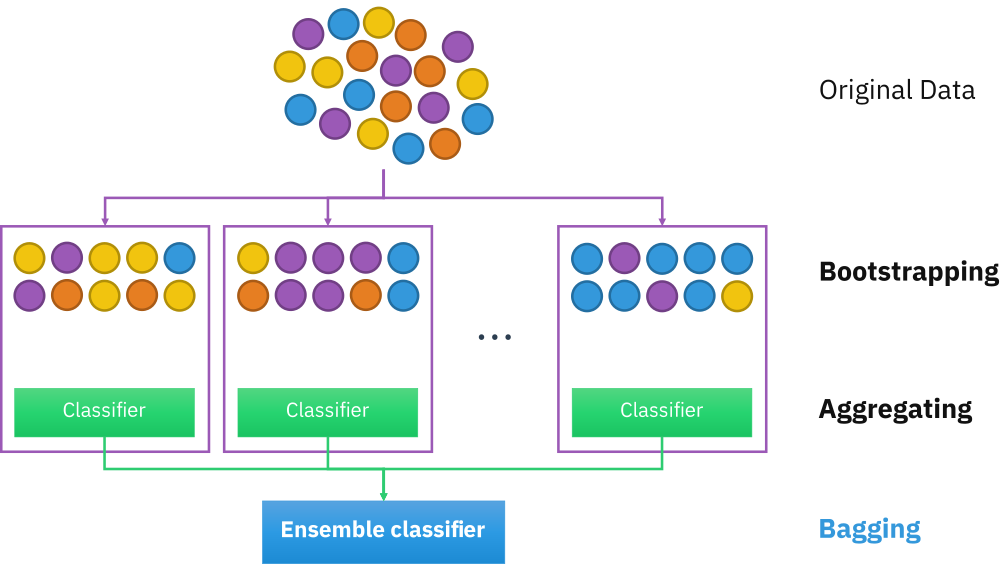
\includegraphics[width=3.5in]{figures/bagging.png}
            \caption{Bagging算法}
            \label{bagging}
            \end{figure}
            \textbf{Bagging}利用\textit{有放回抽样}生成新的训练数据集(Bootstrap samples)。
		\end{frame}

        \begin{frame}
		  \frametitle{\textbf{决策树 (Desicion Tree)}}
            \begin{columns}
                \column{.5\textwidth}
                \footnotesize
                \begin{figure}[!t]
                    \centering
                    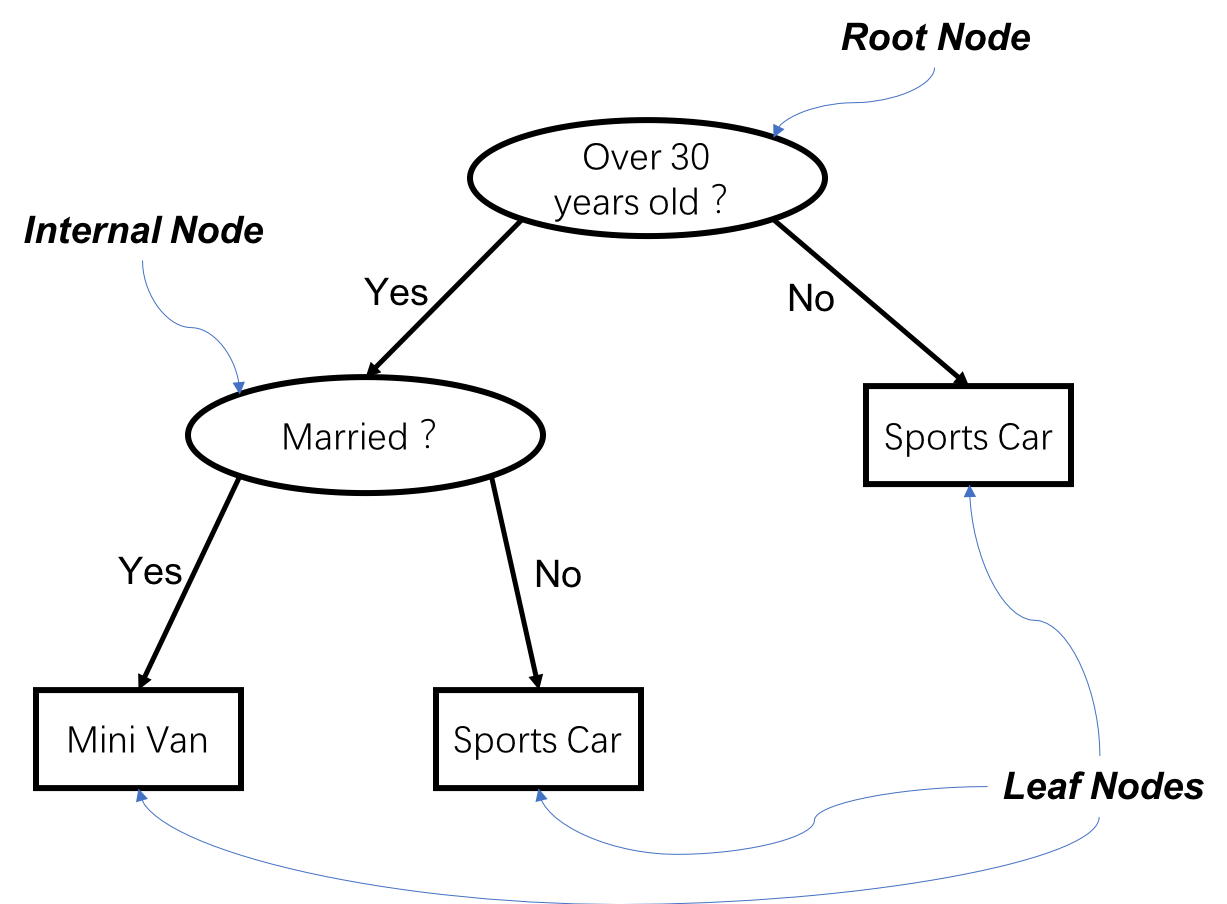
\includegraphics[width=1.1\textwidth]{figures/dt_eg.png}
                    \caption{决策树案例}
                    \label{figure3_OTT}
                \end{figure}

                \column{.5\textwidth}
                \begin{figure}[!t]
                    \centering
                    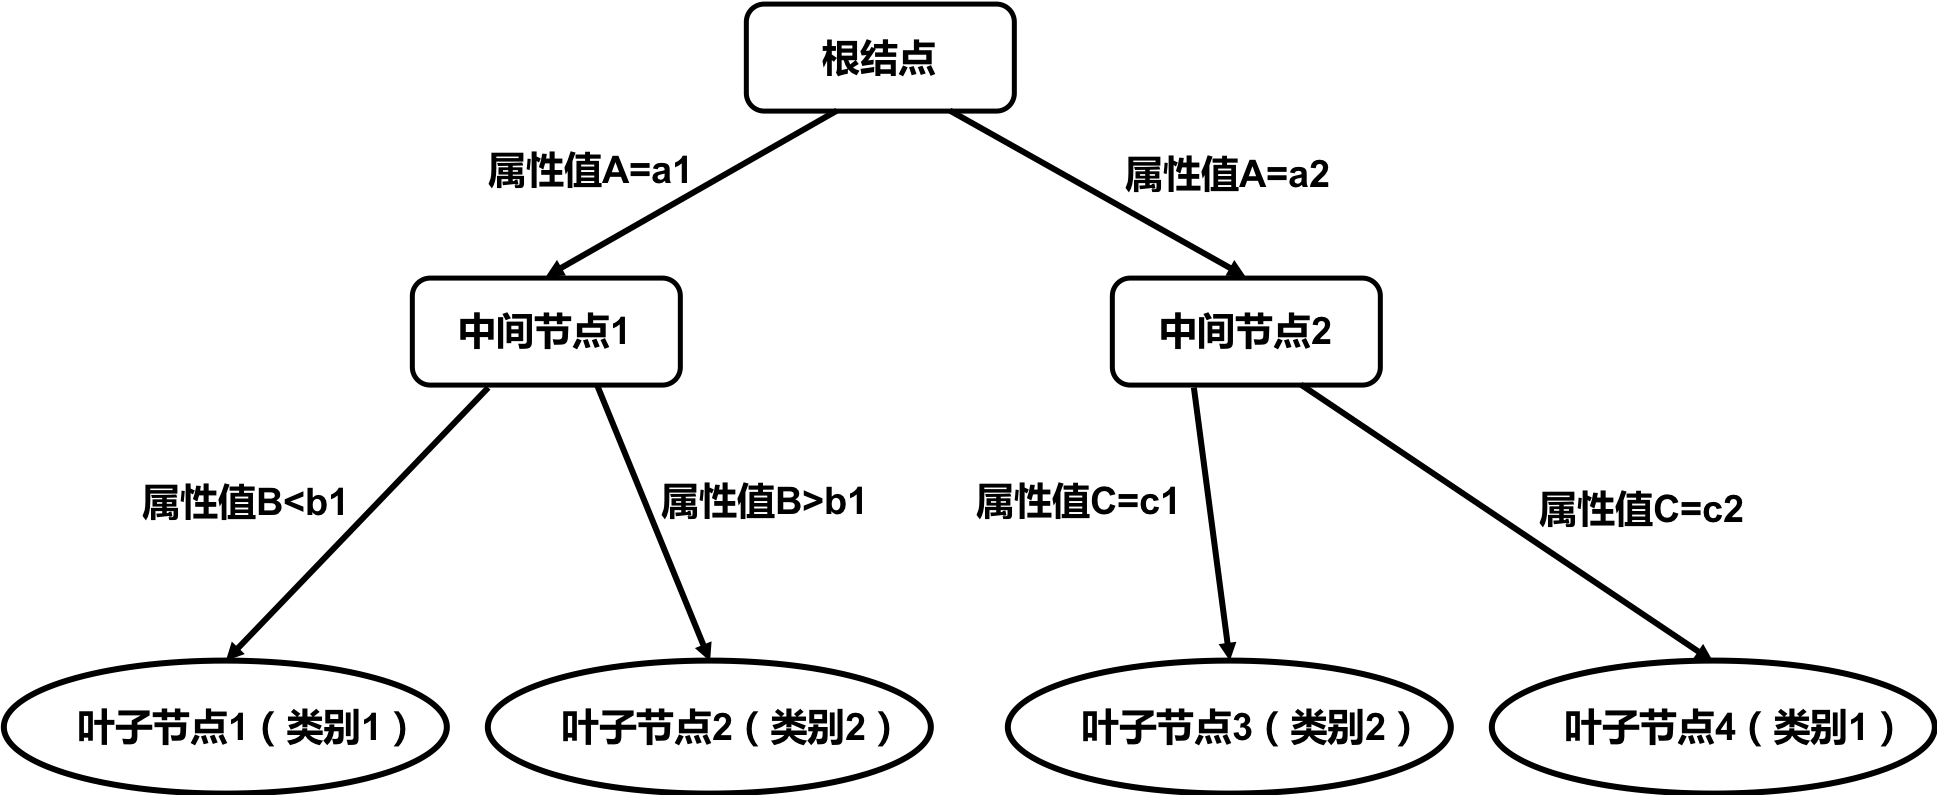
\includegraphics[width=1.1\textwidth]{figures/dt_general.png}
                    \caption{决策树归纳案例}
                    \label{figure3_OTT}
                \end{figure}
            \end{columns}
            决策树的训练:构建一棵决策树(ID3,C4.5,CART)。\\
            决策树的测试:自顶而下匹配一条路径。
        \end{frame}
        
        \begin{frame}
            \frametitle{\textbf{决策树生成算法}}
            \begin{columns}
                \column{.4\textwidth}
                \footnotesize
                \begin{itemize}
                    \item 训练集样本特征:性别、年龄和职业。
                    \item 预测目标:是否喜欢玩电脑游戏。
                    \item 算法关键:每次寻找出当前最佳分割属性。
                \end{itemize}

                \column{.6\textwidth}
                \begin{figure}[!t]
                    \centering
                    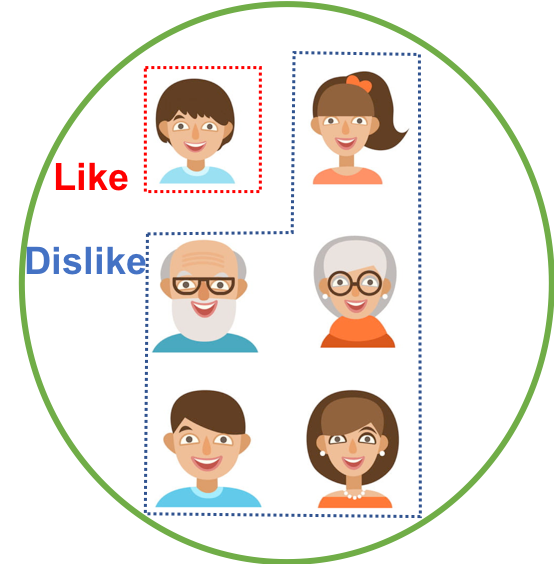
\includegraphics[width=1\textwidth]{figures/dt_gen_0.png}
                \end{figure}
            \end{columns}
        \end{frame}

        \begin{frame}
            \frametitle{\textbf{决策树生成算法}}
            \begin{columns}
                \column{.4\textwidth}
                \footnotesize
                \begin{itemize}
                    \item 训练集样本特征:性别、年龄和职业。
                    \item 预测目标:是否喜欢玩电脑游戏。
                    \item 根据某分割指标,从3个属性中选择\textbf{年龄}作为分割属性,分裂节点。
                    \item 无需分割,则停止分裂节点。
                \end{itemize}

                \column{.6\textwidth}
                \begin{figure}[!t]
                    \centering
                    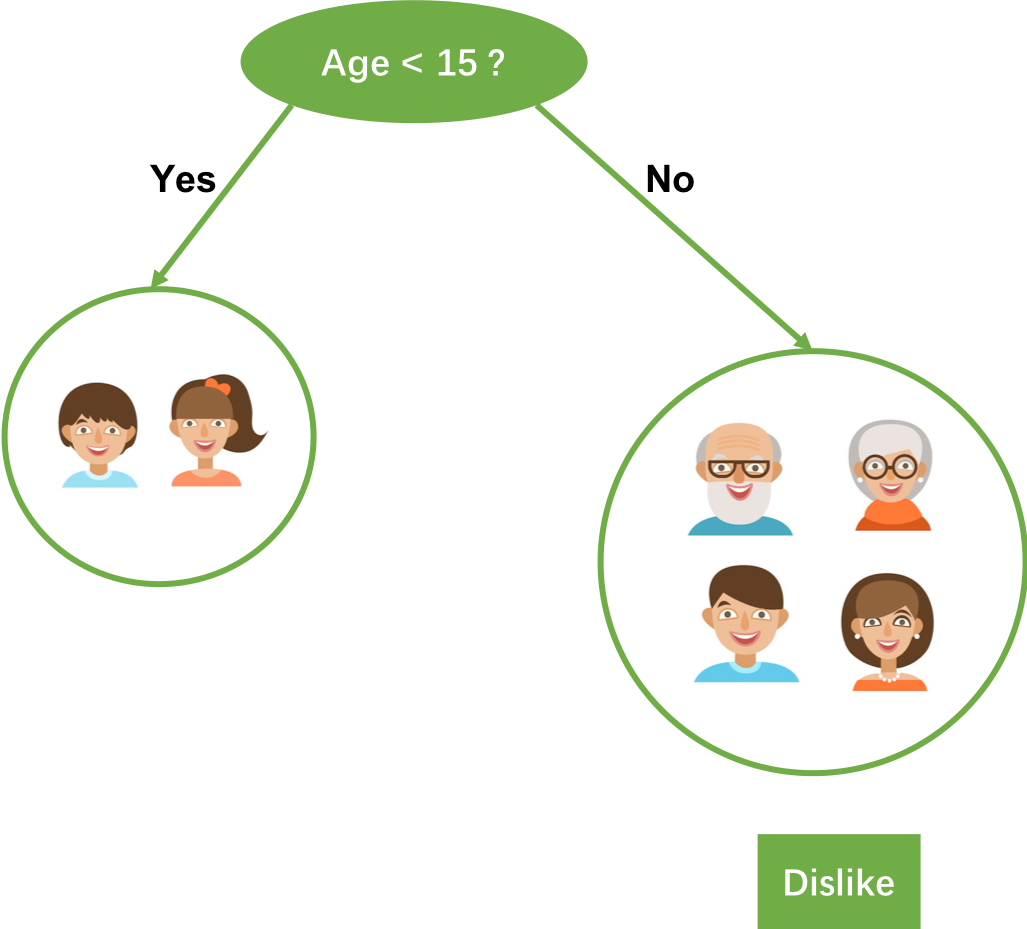
\includegraphics[width=1.1\textwidth]{figures/dt_gen_1.png}
                \end{figure}
            \end{columns}
        \end{frame}

        \begin{frame}
            \frametitle{\textbf{决策树生成算法}}
            \begin{columns}
                \column{.4\textwidth}
                \footnotesize
                \begin{itemize}
                    \item 训练集样本特征:性别、年龄和职业。
                    \item 预测目标:是否喜欢玩电脑游戏。
                    \item 对需要再次分割的节点,根据某分割指标,从剩下的2个属性中选择\textbf{性别}作为分割属性,分裂节点。
                \end{itemize}

                \column{.6\textwidth}
                \begin{figure}[!t]
                    \centering
                    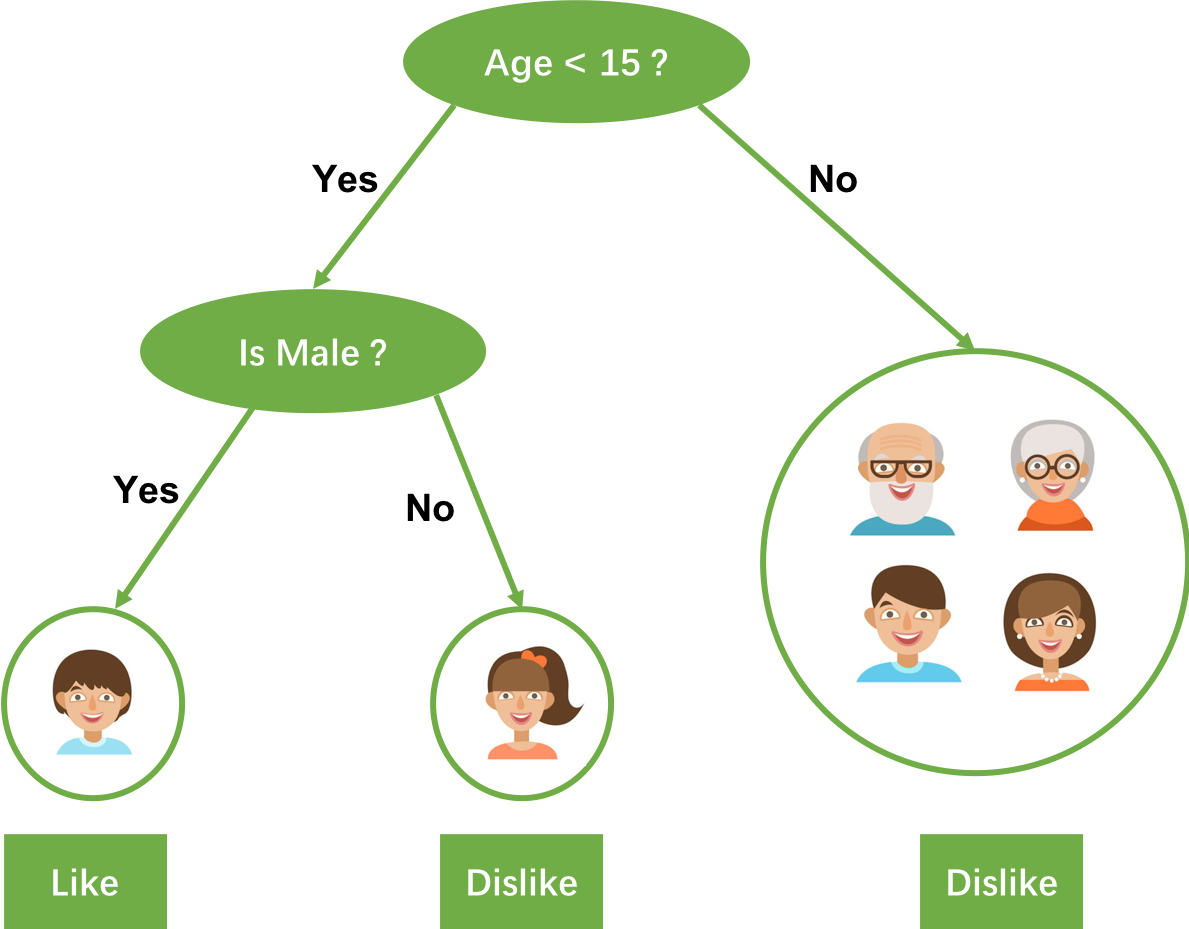
\includegraphics[width=1.1\textwidth]{figures/dt_gen.png}
                \end{figure}
            \end{columns}
        \end{frame}

        \begin{frame}
            \frametitle{\textbf{决策树生成算法}}
            \begin{table}[htbp!]
                \caption{三种最常见的决策树生成算法比较}
                \label{dt_compare}
                \centering
                \begin{tabular}{c c c c c c}
                \hline
                生成算法 & 分割指标  & 支持的属性 & 缺失值处理 \\ \hline
                ID3 & 信息增益 & 仅离散属性 & 不支持\\     
                C4.5 & 信息增益率  & 离散、连续属性 & 支持\\    
                CART & 基尼指数 & 离散、连续属性 & 支持 \\ \hline
                \end{tabular}
            \end{table}
        \end{frame}

        \begin{frame}
            \frametitle{\textbf{随机森林 (Random Forest)}}
            \begin{block}{\textbf{随机森林的随机性}}
                \begin{itemize}
                  \item 随机森林 = Bagging + 决策树(CART)
                  \item 训练集生成的随机性 $\Rightarrow$ Bagging (Bootstrap样本)
                  \item 特征变量选取的随机性 $\Rightarrow$ 决策树生成中,每次分裂节点时,随机选择一部分特征作为候选分割属性,
                    常见$M=\sqrt{N}$,$M=\log _2{N}$,再从候选属性中,寻找出最佳分割属性。
                \end{itemize}
            \end{block}
        \end{frame}

        \begin{frame}
            \frametitle{\textbf{随机森林 (Random Forest)}}
              \begin{columns}
                  \column{.5\textwidth}
                  \footnotesize
                  \begin{figure}[!t]
                      \centering
                      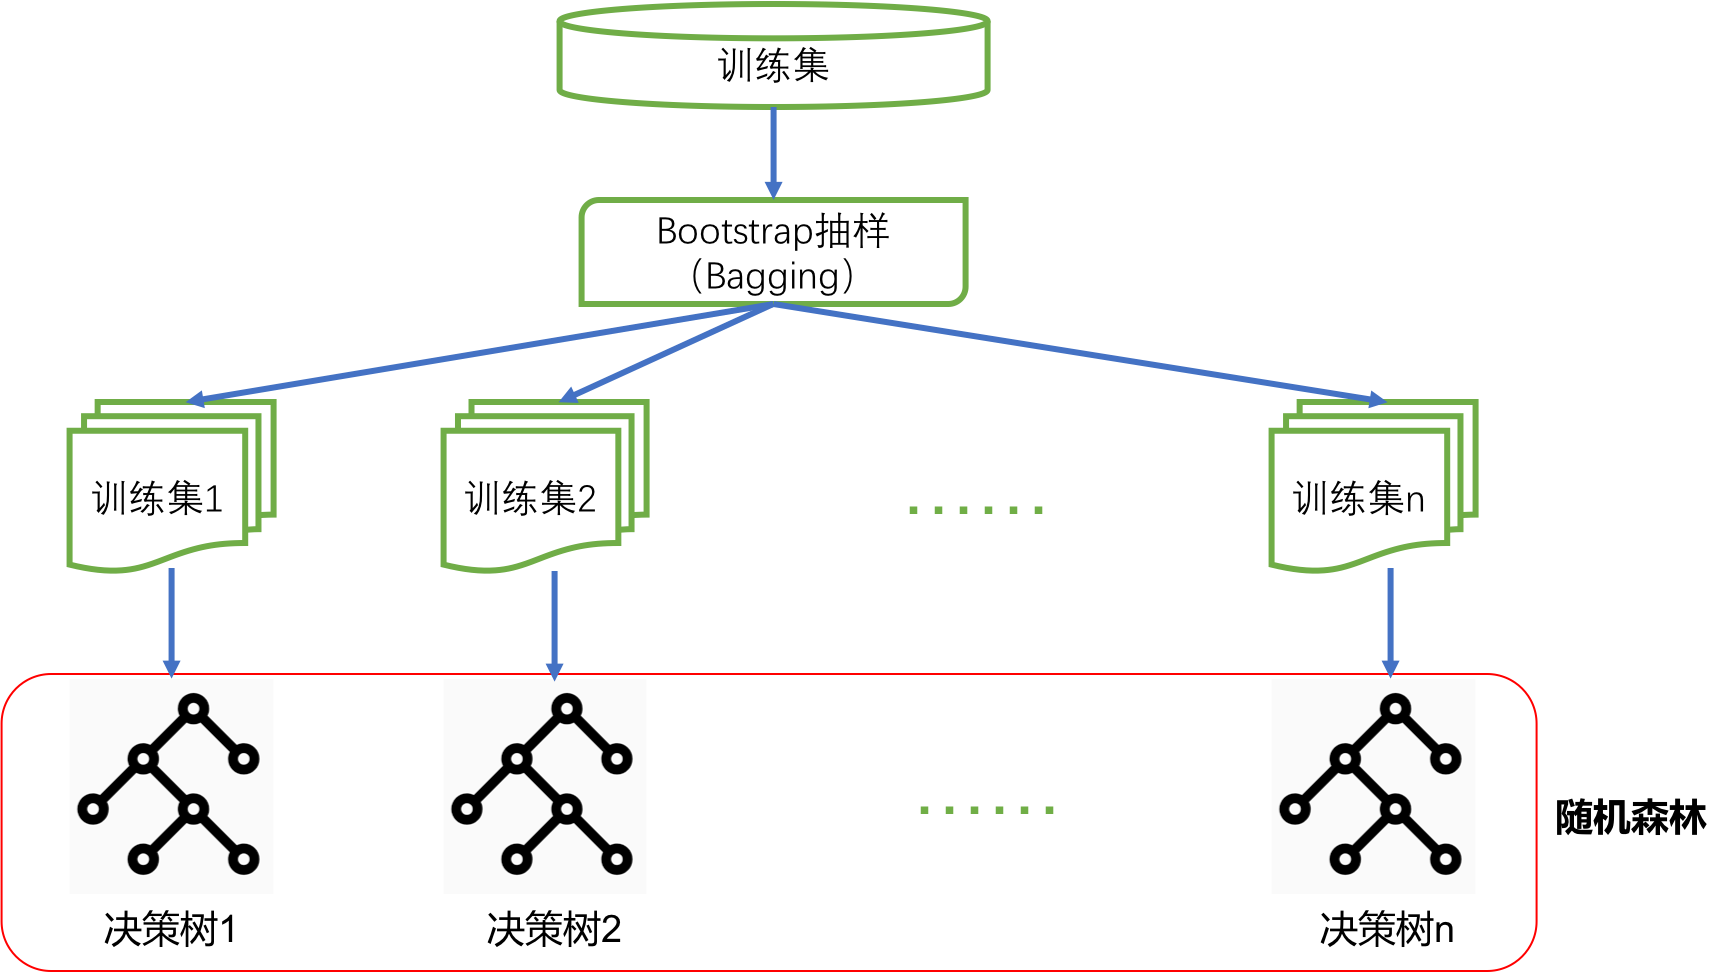
\includegraphics[width=1.15\textwidth]{figures/rf_training.png}
                      \caption{随机森林训练过程}
                  \end{figure}
  
                  \column{.5\textwidth}
                  \begin{figure}[!t]
                      \centering
                      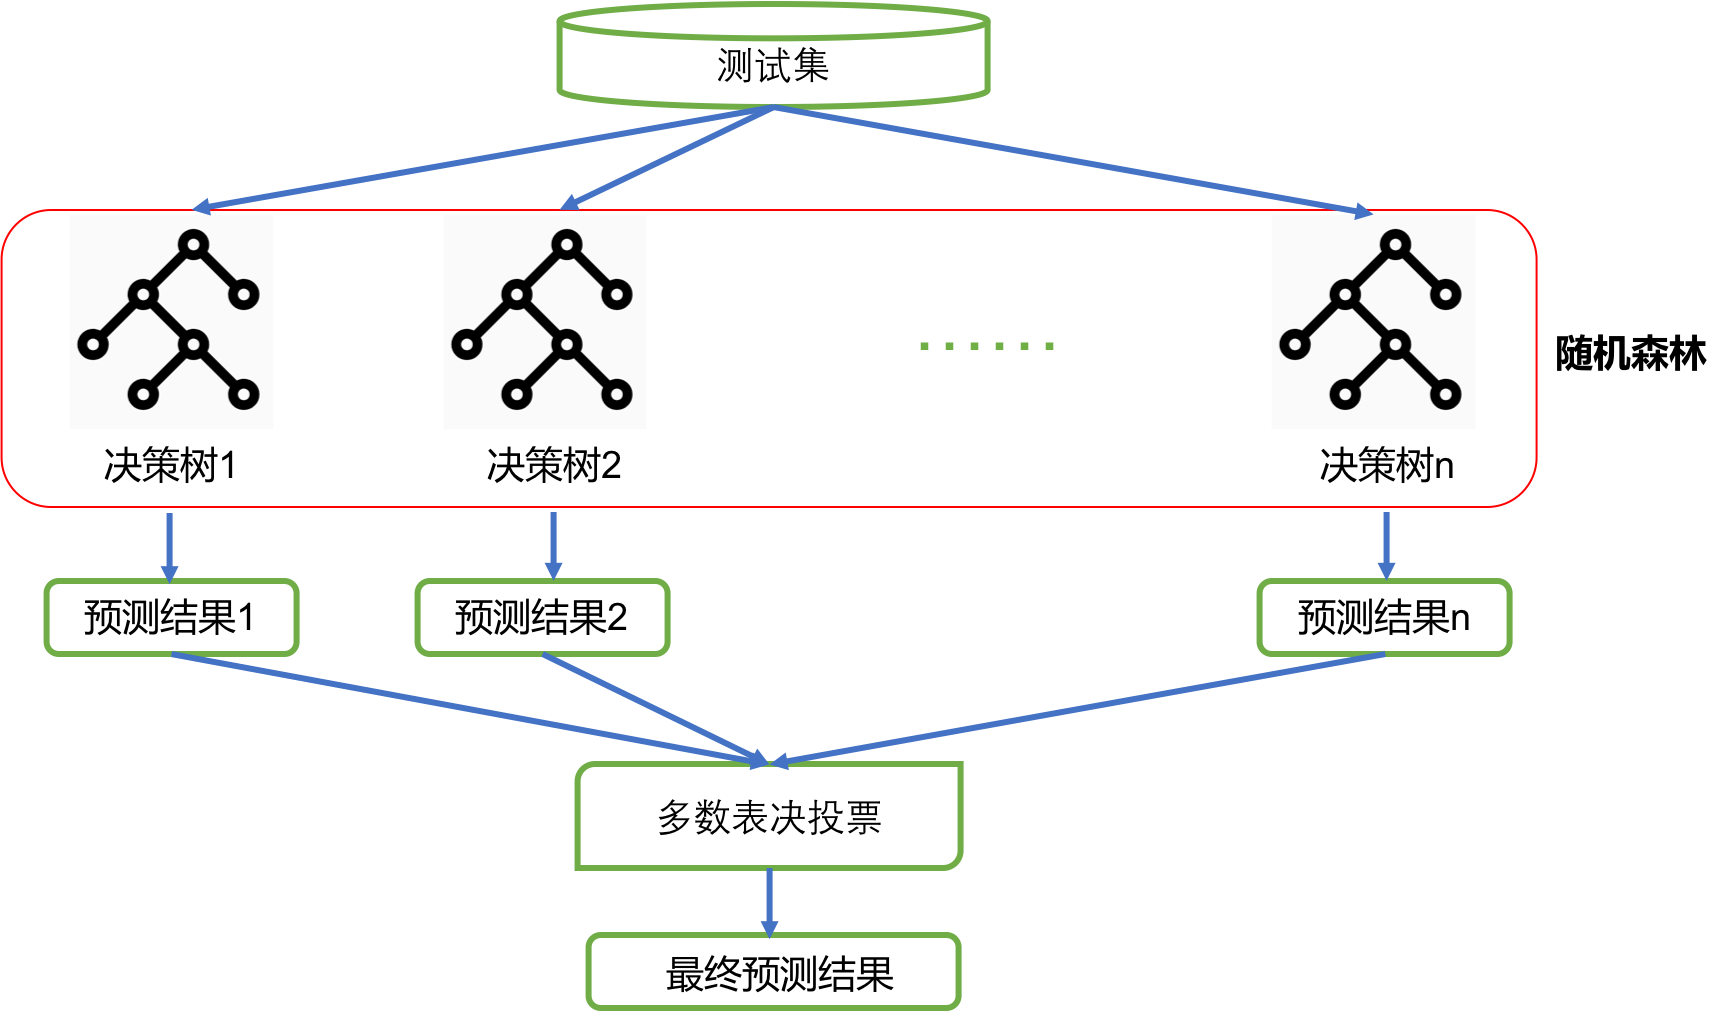
\includegraphics[width=1.1\textwidth]{figures/rf_testing.png}
                      \caption{随机森林测试过程}
                  \end{figure}
              \end{columns}
          \end{frame}

\section[模型]{献血招募模型}


		\begin{frame}
		  \frametitle{\textbf{献血者特征提取}}
            % ----------------分栏的结构开始---------------- %
            % 该结构中使用block分开两个内容区
            % 可根据需要进行图文混排?我还没试过,我想应该可以
            \begin{columns}
                \column{.5\textwidth}
                \footnotesize
                \begin{figure}[!t]
                    \centering
                    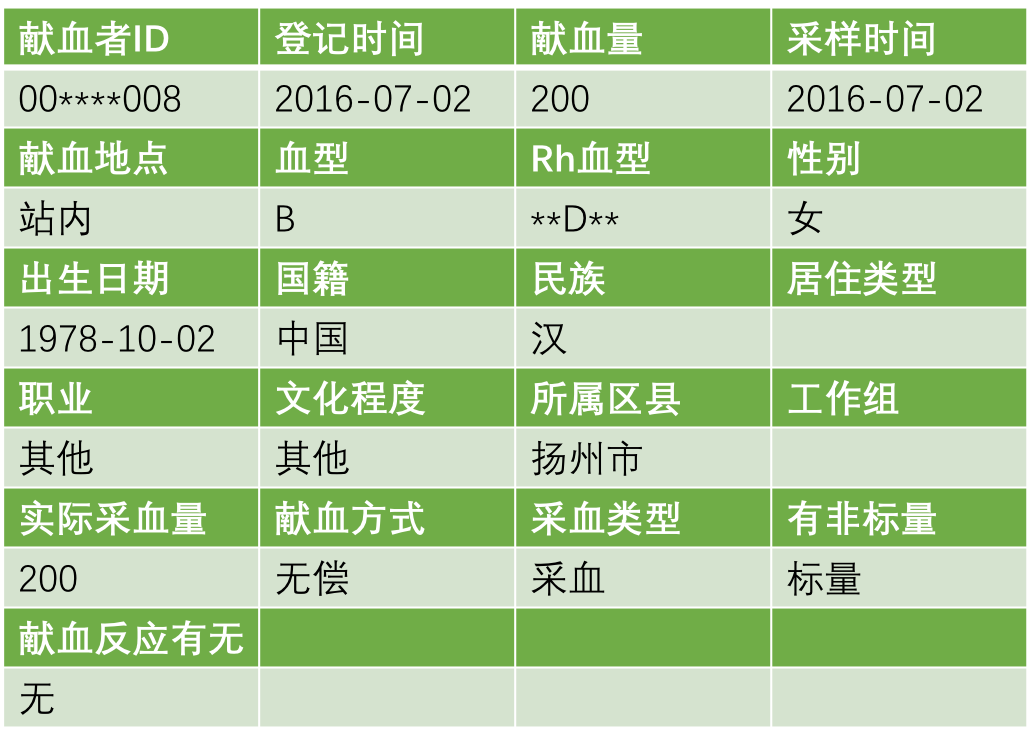
\includegraphics[width=1\textwidth]{figures/record.png}
                    \caption{原始献血记录}
                \end{figure}

                \column{.5\textwidth}
                \begin{figure}[!t]
                    \centering
                    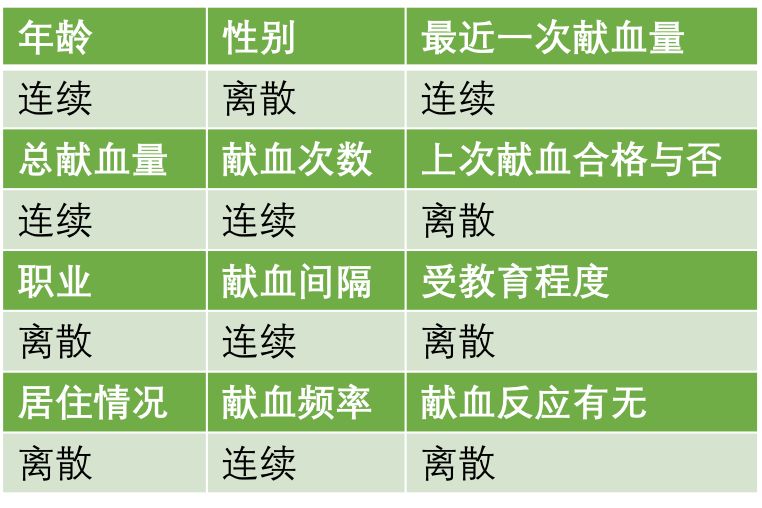
\includegraphics[width=1\textwidth]{figures/feature.png}
                    \caption{特征提取结果}
                \end{figure}
                
            \end{columns}

		\end{frame}

        \begin{frame}
		  \frametitle{\textbf{决策树和随机森林的实现}}
            \begin{block}{\textbf{主要贡献}}
                \begin{itemize}
                    \item 利用层次遍历的思想,将主流的递归版本的决策树生成算法转化为非递归版本。
                    \item 利用graphviz,将决策树和随机森林可视化。
                    \item 利用UCI公开数据集,初步评测了模型性能。
                \end{itemize}
            \end{block}

            \begin{table}[]
                \caption{3种决策树时间性能比较(UCI数据集)}
                \label{dt_time_compare}
                \centering
                \begin{tabular}{cccc}
                \hline
                算法版本 & ID3 (ms)             & C4.5 (ms)            & CART (ms)            \\ \hline
                递归   & 342.64±7.23          & 225.36±4.68          & 285.41±10.23         \\
                非递归  & \textbf{213.45±6.13} & \textbf{121.39±8.09} & \textbf{135.67±8.79} \\ \hline
                提升率  & 37.70\%              & 46.13\%              & 52.64\%              \\ \hline
                \end{tabular}
            \end{table}

        \end{frame}
        
        \begin{frame}
		  \frametitle{\textbf{决策树和随机森林的实现}}
          \begin{figure}[!t]
            \centering
            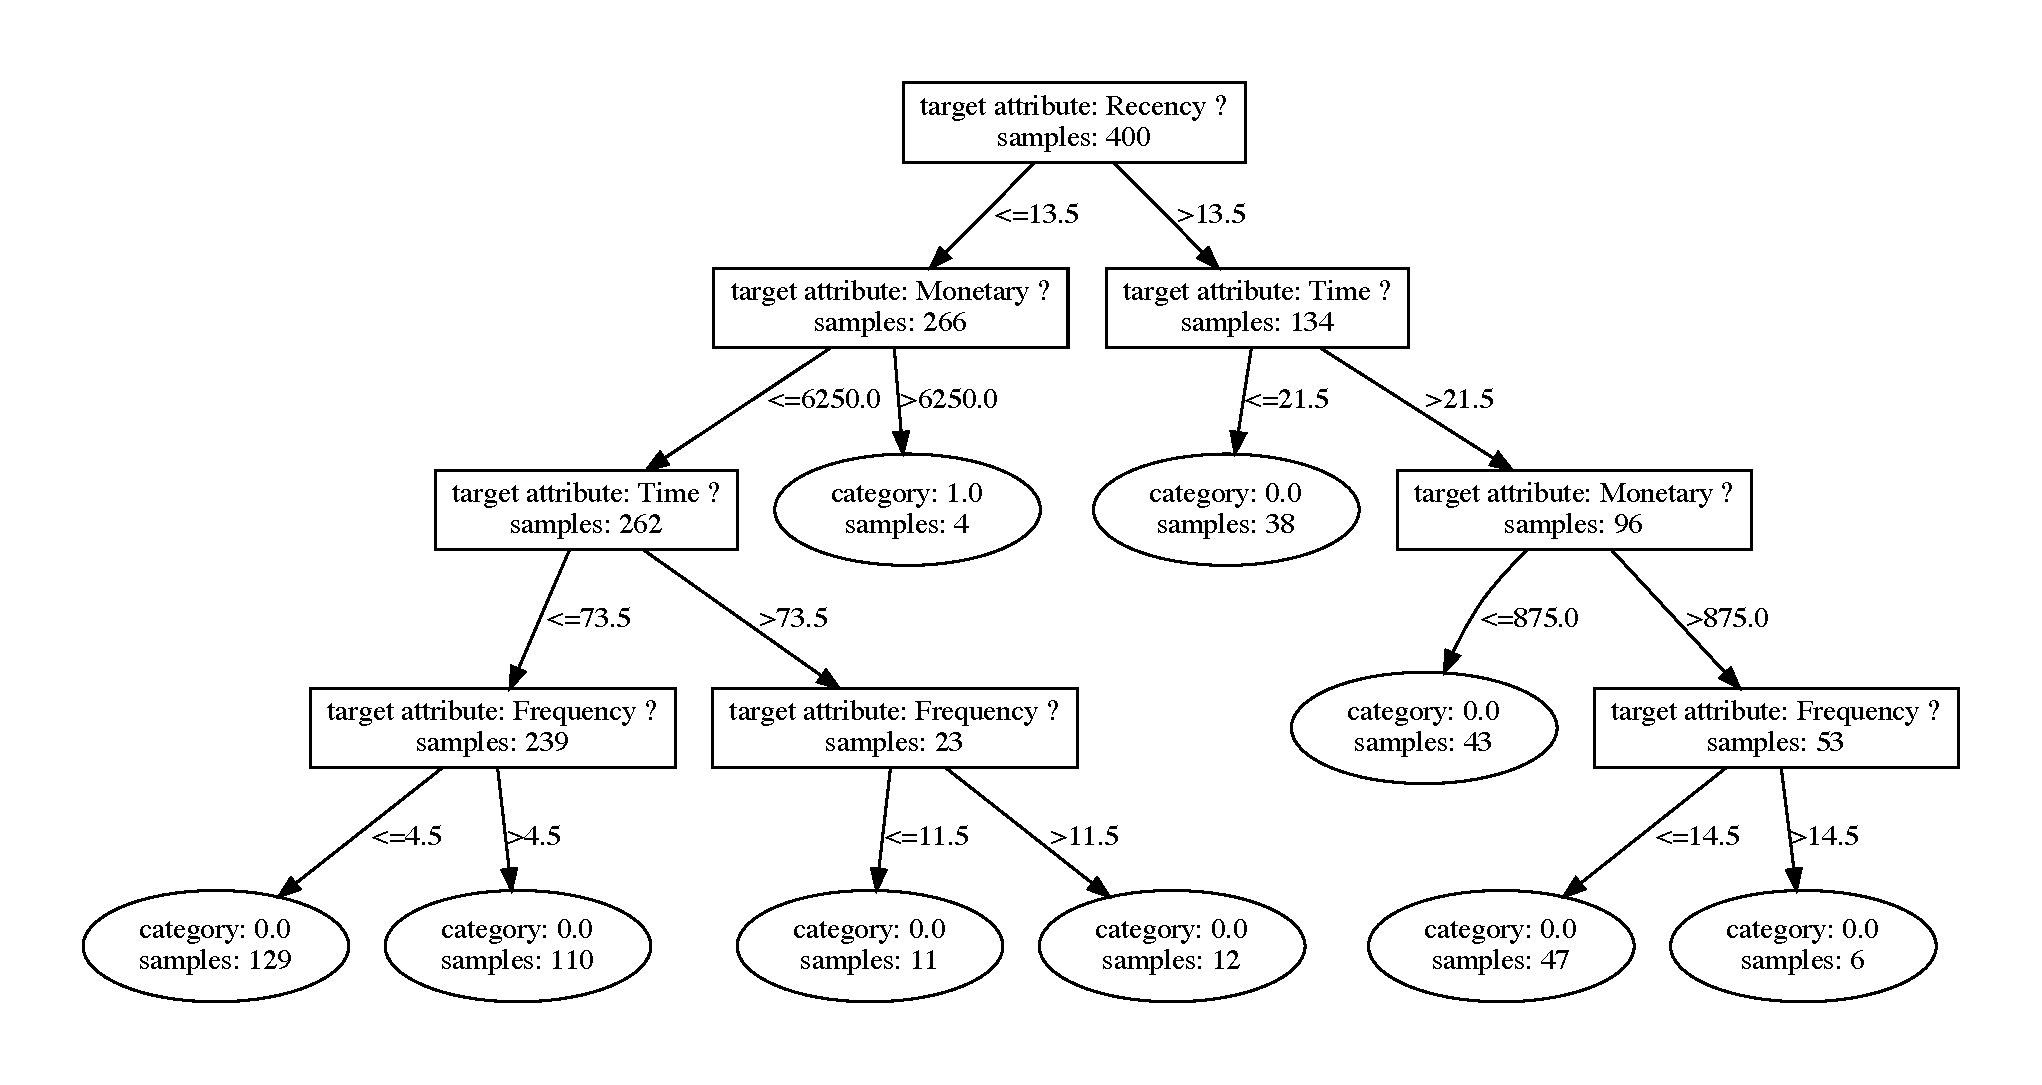
\includegraphics[width=1.1\textwidth]{figures/test_3_random_decision_tree_0.pdf}
            \caption{训练的随机森林中的某棵决策树可视化(UCI数据集)}
        \end{figure}
		\end{frame}

\section[实验]{实验分析}

		\begin{frame}
		  \frametitle{\textbf{数据集特征分布分析}}
		  \begin{block}{\textbf{特征分布}}
                \begin{itemize}
                    \item 绘制了箱形图(Box-whisker Plot)和直方图(Histogram)。
                    \item 利用核密度估计(Kernel Density Estimation)
                    绘制出了变量的概率密度函数。
                \end{itemize}
            \end{block}
            \begin{columns}
                \column{.5\textwidth}
                \begin{figure}
                    \centering
                    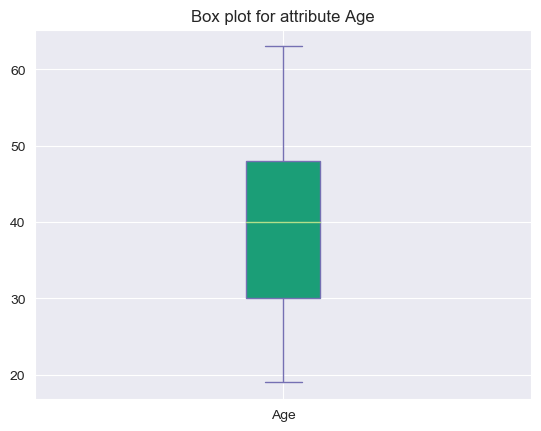
\includegraphics[width=1\textwidth]{figures/age.png}
                    \caption{特征\textbf{年龄}的箱形图(UCI数据集)}
                \end{figure}

                \column{.5\textwidth}
                \begin{figure}
                    \centering
                    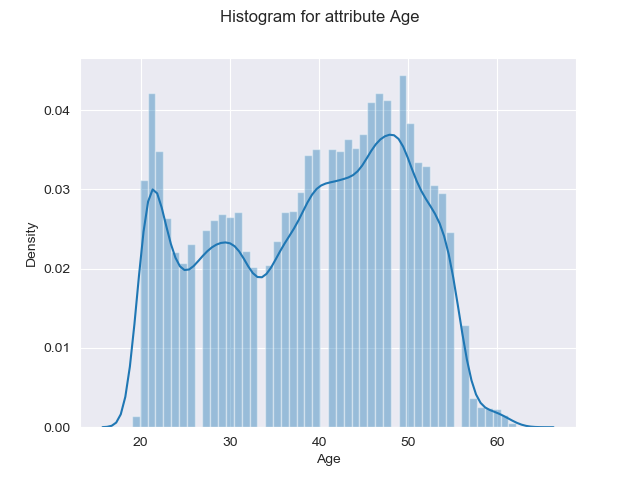
\includegraphics[width=1\textwidth]{figures/dis_Age.png}
                    \caption{特征\textbf{年龄}的直方图(UCI数据集)}
                \end{figure}
            \end{columns}
		\end{frame}

        \begin{frame}
		  \frametitle{\textbf{超参数分析}}
            \begin{block}{\textbf{内部超参数}}
                \begin{itemize}
                    \item 基分类器的数量。
                    \item 决策树生成算法。(ID3,C4.5,CART算法)
                    \item 分裂节点时选择特征的比例公式。($M=\sqrt{N}$,$M=\log _{2}{N}$和$M=N$)
                \end{itemize}
            \end{block}

            \begin{block}{\textbf{外部超参数}}
                \begin{itemize}
                    \item 训练样本的数量。
                \end{itemize}
            \end{block}
		\end{frame}

		\begin{frame}
		  \frametitle{\textbf{内部超参数分析}}
            \begin{columns}
                \column{.5\textwidth}
                \begin{figure}
                    \centering
                    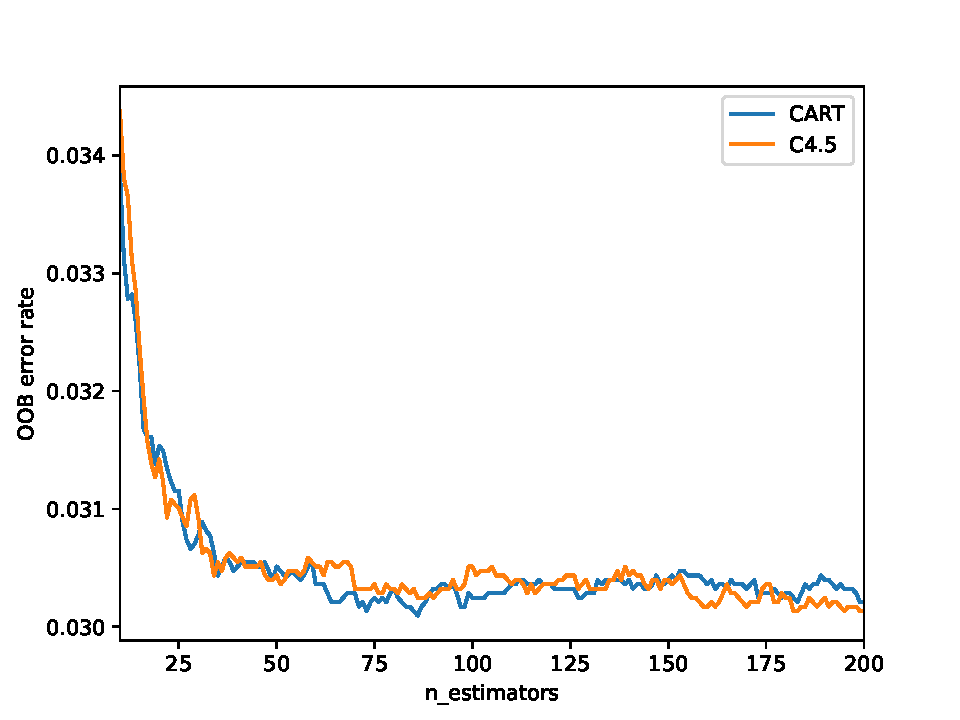
\includegraphics[width=1\textwidth]{figures/hyperpara_criterion_oob_2.pdf}
                    \caption{基分类器数目和决策树生成算法对OOB错误率的影响}
                \end{figure}

                \column{.5\textwidth}
                \begin{figure}
                    \centering
                    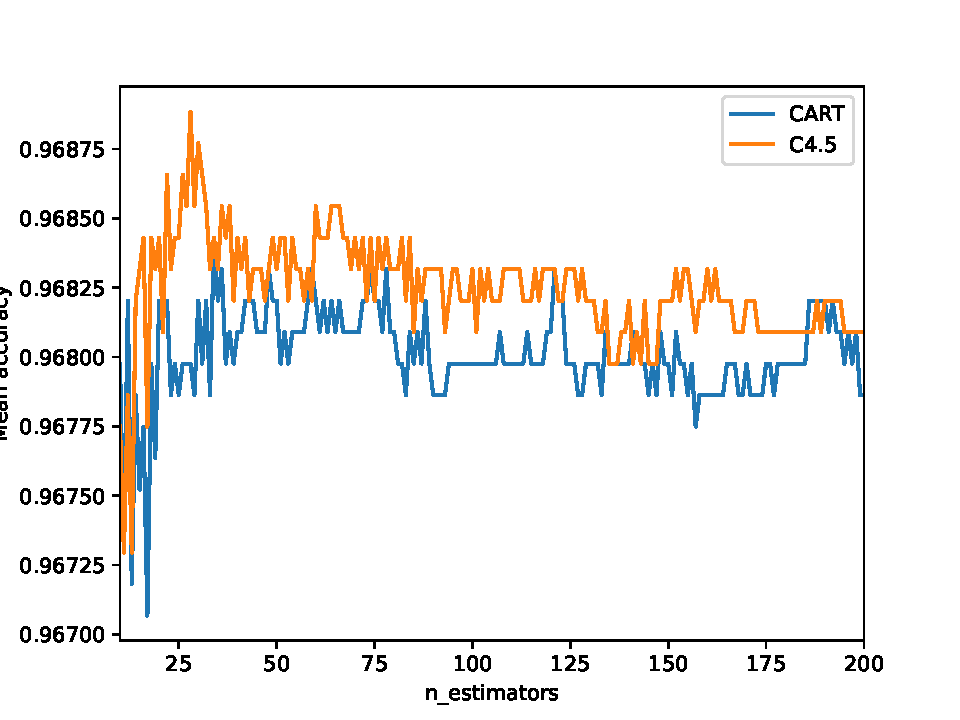
\includegraphics[width=1\textwidth]{figures/hyperpara_criterion_mean_acc_2.pdf}
                    \caption{基分类器数目和决策树生成算法对预测精度的影响}
                \end{figure}
            \end{columns}
        \end{frame}
        
        \begin{frame}
            \frametitle{\textbf{内部超参数分析}}
              \begin{columns}
                  \column{.5\textwidth}
                  \begin{figure}
                      \centering
                      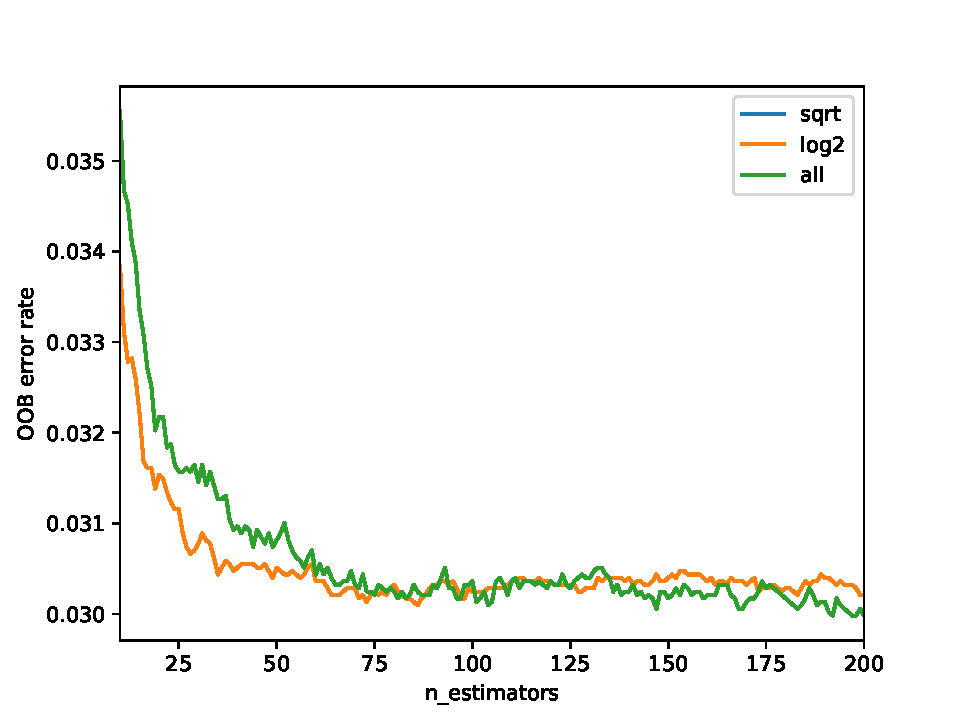
\includegraphics[width=1\textwidth]{figures/hyperpara_max_features_oob_2.pdf}
                      \caption{基分类器数目和节点分裂时特征选择比例对OOB错误率的影响}
                  \end{figure}
  
                  \column{.5\textwidth}
                  \begin{figure}
                      \centering
                      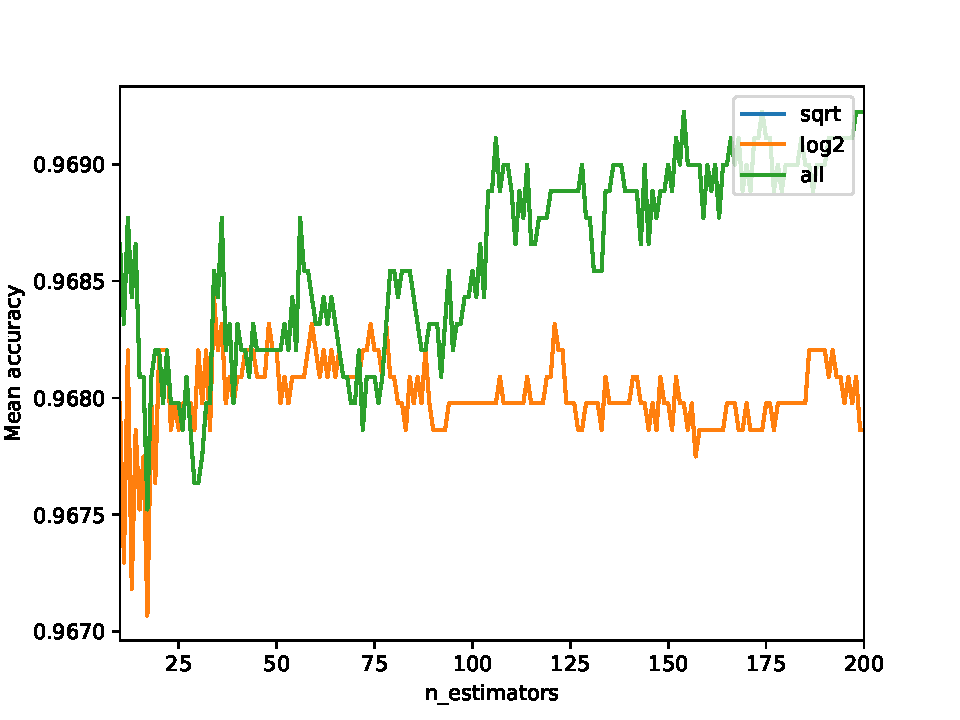
\includegraphics[width=1\textwidth]{figures/hyperpara_max_features_mean_acc_2.pdf}
                      \caption{基分类器数目和节点分裂时特征选择比例对预测精度的影响}
                  \end{figure}
              \end{columns}
          \end{frame}

          \begin{frame}
            \frametitle{\textbf{模型性能比较分析}}
            \begin{table}[]
                \caption{随机森林在真实数据集上性能比较(与其他集成学习算法比较)}
                \label{compare_ensemble}
                \centering
                \begin{tabular}{ccc}
                \hline
                算法                    & 准确率     \\ \hline
                Decision Tree         & 0.929±0.042          \\ 
                Bagging+Decision Tree & 0.956±0.039          \\
                AdaBoost              & 0.950±0.032          \\
                Gradient Boosting     & 0.959±0.040          \\ \hline
                Random Forest         & \textbf{0.969±0.039} \\ \hline
                \end{tabular}
            \end{table}

            \begin{table}[]
                \caption{随机森林在真实数据集上性能比较(与其他分类算法比较)}
                \label{compare_other}
                \centering
                \begin{tabular}{ccc}
                \hline
                算法             & 准确率                      \\ \hline
                SVM            & 0.952±0.042          \\
                KNN            & 0.943±0.004        \\
                Neural network & 0.941±0.002         \\
                SGD            & 0.952±0.142         \\ \hline
                Random Forest             & \textbf{0.969±0.039} \\ \hline
                \end{tabular}
            \end{table}

          \end{frame}

          \begin{frame}
            \frametitle{\textbf{模型性能比较分析}}
            \begin{figure}[htbp!]
                \centering 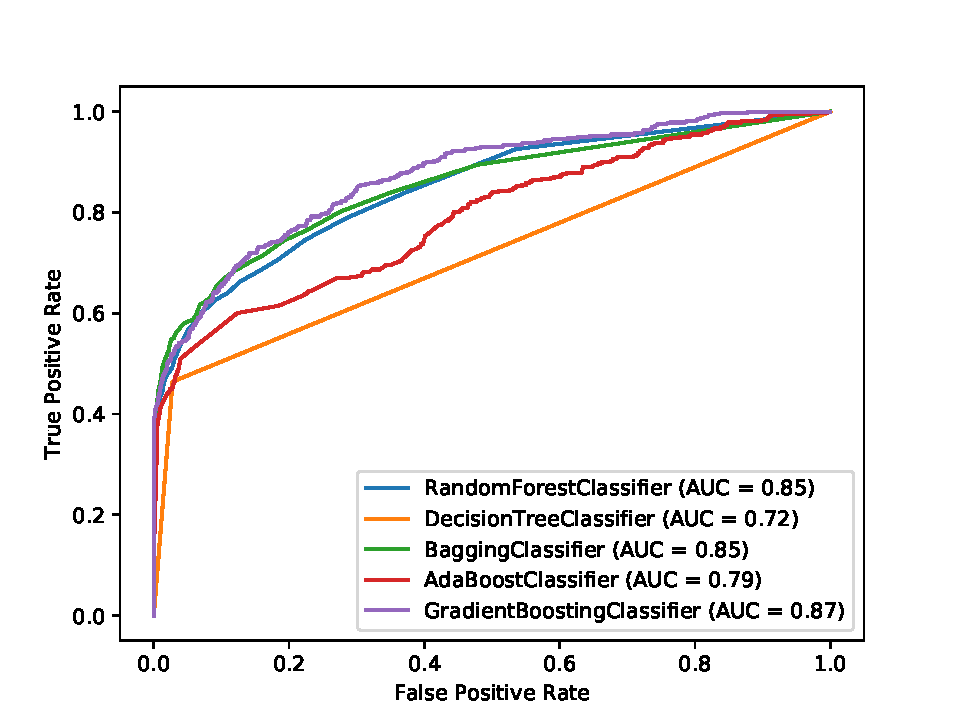
\includegraphics[width=0.8\textwidth]{figures/intra_whole_roc.pdf} 
                \caption{表\ref{compare_ensemble}中对应算法的ROC曲线比较}
            \end{figure}
          \end{frame}

          \begin{frame}
            \frametitle{\textbf{模型性能比较分析}}
            \begin{figure}[htbp!]
                \centering 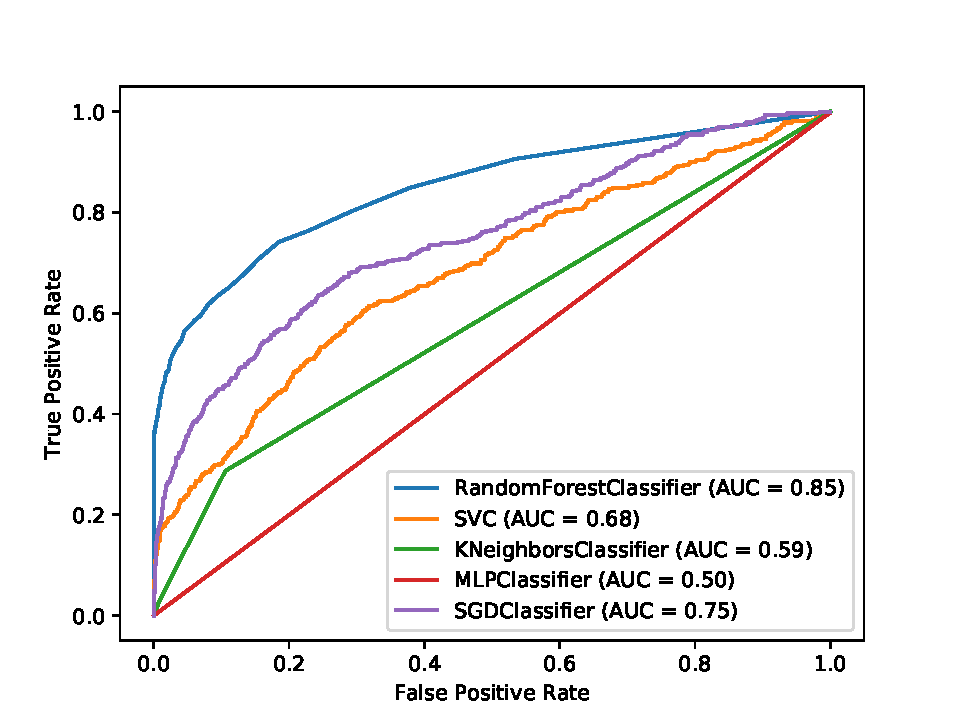
\includegraphics[width=0.8\textwidth]{figures/inter_whole_roc.pdf} 
                \caption{表\ref{compare_other}中对应算法的ROC曲线比较}
            \end{figure}
          \end{frame}
\section[结论]{总结}

		\begin{frame}
		  \frametitle{\textbf{结论}}
          \begin{enumerate}
            \item 将随机森林算法引入到献血者招募问题当中,
            给出了一种利用机器学习技术辅助医护人员进行精准招募的方法,
            提升了招募精度,降低了招募成本。
            \item 对当前学术界医疗和机器学习相关技术进行了全面而深入的文献调研
            工作,总结了近年来医疗AI的发展趋势。
            \item 改进了三种主流的经典决策树生成算法:ID3、C4.5和CART,
            将递归版本转化成非递归版本,降低了时空开销,为随机森林的算法
            实现提供了基础。
            \item 通过超参数调整,将模型的最终精度提升到了95\%以上,
            并进行了详尽全面的模型比较分析。
        \end{enumerate}
        
		\end{frame}


\section*{}
            \begin{frame}

                \begin{center}
                    \begin{minipage}{1\textwidth}
                        \setbeamercolor{mybox}{fg=white, bg=black!60!green}
                        \begin{beamercolorbox}[wd=0.70\textwidth, rounded=true, shadow=true]{mybox}
                        \LARGE \centering Thanks for Listening.
                        \end{beamercolorbox}
                    \end{minipage}
                \end{center}

            \end{frame}

\end{document} 